% Drawing 23/04-2 -- folder 23, batch 04, archive page 77 (PDF page 78).
% Transcription: croquis au crayon, au-dessus du trait : un $X'$ biffé d'où partent deux flèches vers $Y$, trois $\Omega$ dont un biffé, et un mot illisible sous le trait
% Kind: pencil sketch above a line: X' struck, arrows, Omegas, diagonal strokes. Method 2 (schematic redraw from the facsimile). Status: partial.
% Notes: Pencil: a struck X' (with an X above it) from which two arrows go right towards Y (placed after the transcription), three long diagonal strokes down to a horizontal line, the labels Omega^1, Omega^1_{X'/Y'} with a struck symbol and a dash before it, and Omega^1_{X/Y} lower left. A small square Y~ - X~ over Y - X at the top left, also pencil, is drawn. The word under the line is not read and left out; the typed text showing through from the back is not reproduced. Labels are approximate readings.
% Coordinates: 1 unit = 1 mm = 1/100 of the crop width (bbox in page fractions: [0.06, 0.05, 0.96, 0.34]).
% Redrawn by Claude (claude-opus-5-5), issue #73, 2026-11-07; not checked by a human; not compiled (no TeX in the session).
% Rights: reproduces part of the work -- behind RENDER_TRANSCRIPTS, never published by itself.
\documentclass[tikz,border=3pt]{standalone}
\usepackage{amsmath,amssymb}
\usetikzlibrary{patterns,arrows.meta}
\tikzset{pencil/.style={black!45}, struck/.style={black!35}, mark/.style={circle,draw,inner sep=1.3pt}, pt/.style={circle,fill,inner sep=0.9pt}, opt/.style={circle,draw,fill=white,inner sep=1.1pt}}
\begin{document}
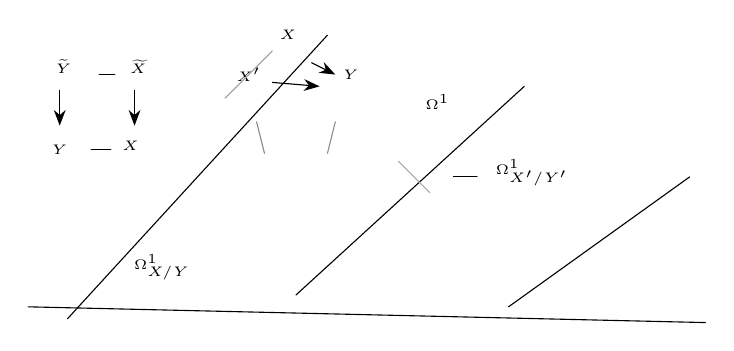
\begin{tikzpicture}[x=1mm,y=1mm,line cap=round,line join=round,font=\scriptsize]
\node[inner sep=1pt] at (13.5,-10) {\tiny $\widetilde{Y}$};
\draw (18,-11) -- (20,-11);
\node[inner sep=1pt] at (23,-10) {\tiny $\widetilde{X}$};
\draw[-{Stealth[length=2mm]}] (13,-13) -- (13,-17.5);
\draw[-{Stealth[length=2mm]}] (22.5,-13) -- (22.5,-17.5);
\node[inner sep=1pt] at (13,-20.5) {\tiny $Y$};
\draw (17,-20.5) -- (19.5,-20.5);
\node[inner sep=1pt] at (22,-20) {\tiny $X$};
\node[inner sep=1pt] at (37,-11) {\tiny $X'$};
\draw[struck] (34,-14) -- (40,-8);
\node[inner sep=1pt] at (42,-6) {\tiny $X$};
\draw[-{Stealth[length=2mm]}] (40,-12) -- (46,-12.5);
\draw[-{Stealth[length=2mm]}] (45,-9.5) -- (48,-11);
\node[inner sep=1pt] at (50,-11) {\tiny $Y$};
\draw (14,-42) -- (47,-6);
\draw (43,-39) -- (72,-12.5);
\draw (70,-40.5) -- (93,-24);
\draw (9,-40.5) -- (95,-42.5);
\node[inner sep=1pt] at (61,-14.5) {\tiny $\Omega^1$};
\draw[struck] (56,-22) -- (60,-26);
\draw (63,-24) -- (66,-24);
\node[inner sep=1pt] at (73,-23.5) {\tiny $\Omega^1_{X'/Y'}$};
\node[inner sep=1pt] at (26,-35.5) {\tiny $\Omega^1_{X/Y}$};
\draw[pencil] (38,-17) -- (39,-21);
\draw[pencil] (48,-17) -- (47,-21);
\end{tikzpicture}
\end{document}
